\chapter{Ground-based gammma-ray detection}
\label{CHAP::TECHNIQUE}

\section{Extensive Air-Showers}
\label{SEC::TECHNIQUE::SHOWERS}

Discovered in 1938 by Pierre Auger, Extensive Air-Showers (E.A.S.) are
cascades of high energy photons, electrons and positrons initiated by
cosmic-rays or \Grays interacting in the upper atmosphere. Typically,
the primary particle interacts at an altitude between $15-30$\,km
producing secondary particles which continue to interact in the
increasingly dense atmosphere through bremsstrahlung and
pair-production, producing a cascade of particles in the
atmosphere. The number of particles in the cascade continues to
increase until their average energy reaches a critical value, at which
ionization becomes the dominant interaction mode ($\sim$100\,MeV in
air); the cascade subsequently dies rapidly. The point in the
development of the cascade at which ionization becomes dominant at
which the number of charged particles in the shower is greatest is
referred to as ``shower maximum''. In general, very energetic
primaries produce showers with larger numbers of secondary particles
and the shower maximum occurs deeper into the atmosphere. For
primaries with sufficiently large energy the cascade can reach ground
level before the critical energy is reached and the shower can be
detected directly using charged-particle detectors, such as
scintillators, at ground level. Placing these detectors on the highest
mountains lowers the energy a primary must have to be
detected. Showers from lower energy primaries typically die out
completely before they reach ground level, and hence are impossible to
detect directly from the ground.  Figure~\ref{FIG::TECHNIQUE::SHOWERS}
shows the profile in the atmosphere of the charged particles in two
{\Grayc}-induced air-showers. The first, initiated by a 100\,GeV
photon, dies out before it reaches ground level. Charged particles
from the second, induced by a 1\,TeV photon, reach ground level in an
area of diameter $\sim$200\,m. It was the coincidental detection of
charged particles at two locations, separated by such large distances
on the ground, that led Auger to the discovery of E.A.S. Modern
instruments for detecting these cascades directly on the ground
consist of arrays of charged particle detectors covering a large
ground region. One such example is the Pierre Auger Observatory being
built in Argentina which will consist of 1600 water \Cerenkov
detectors distributed over an area of 3,000\,km$^2$
\citep{REF::AUGER::1996PROPOSAL}.

\begin{figure}[t]
\centerline{\resizebox{\textwidth}{!}{\resizebox*{!}{\textheight}{\rotatebox{270}{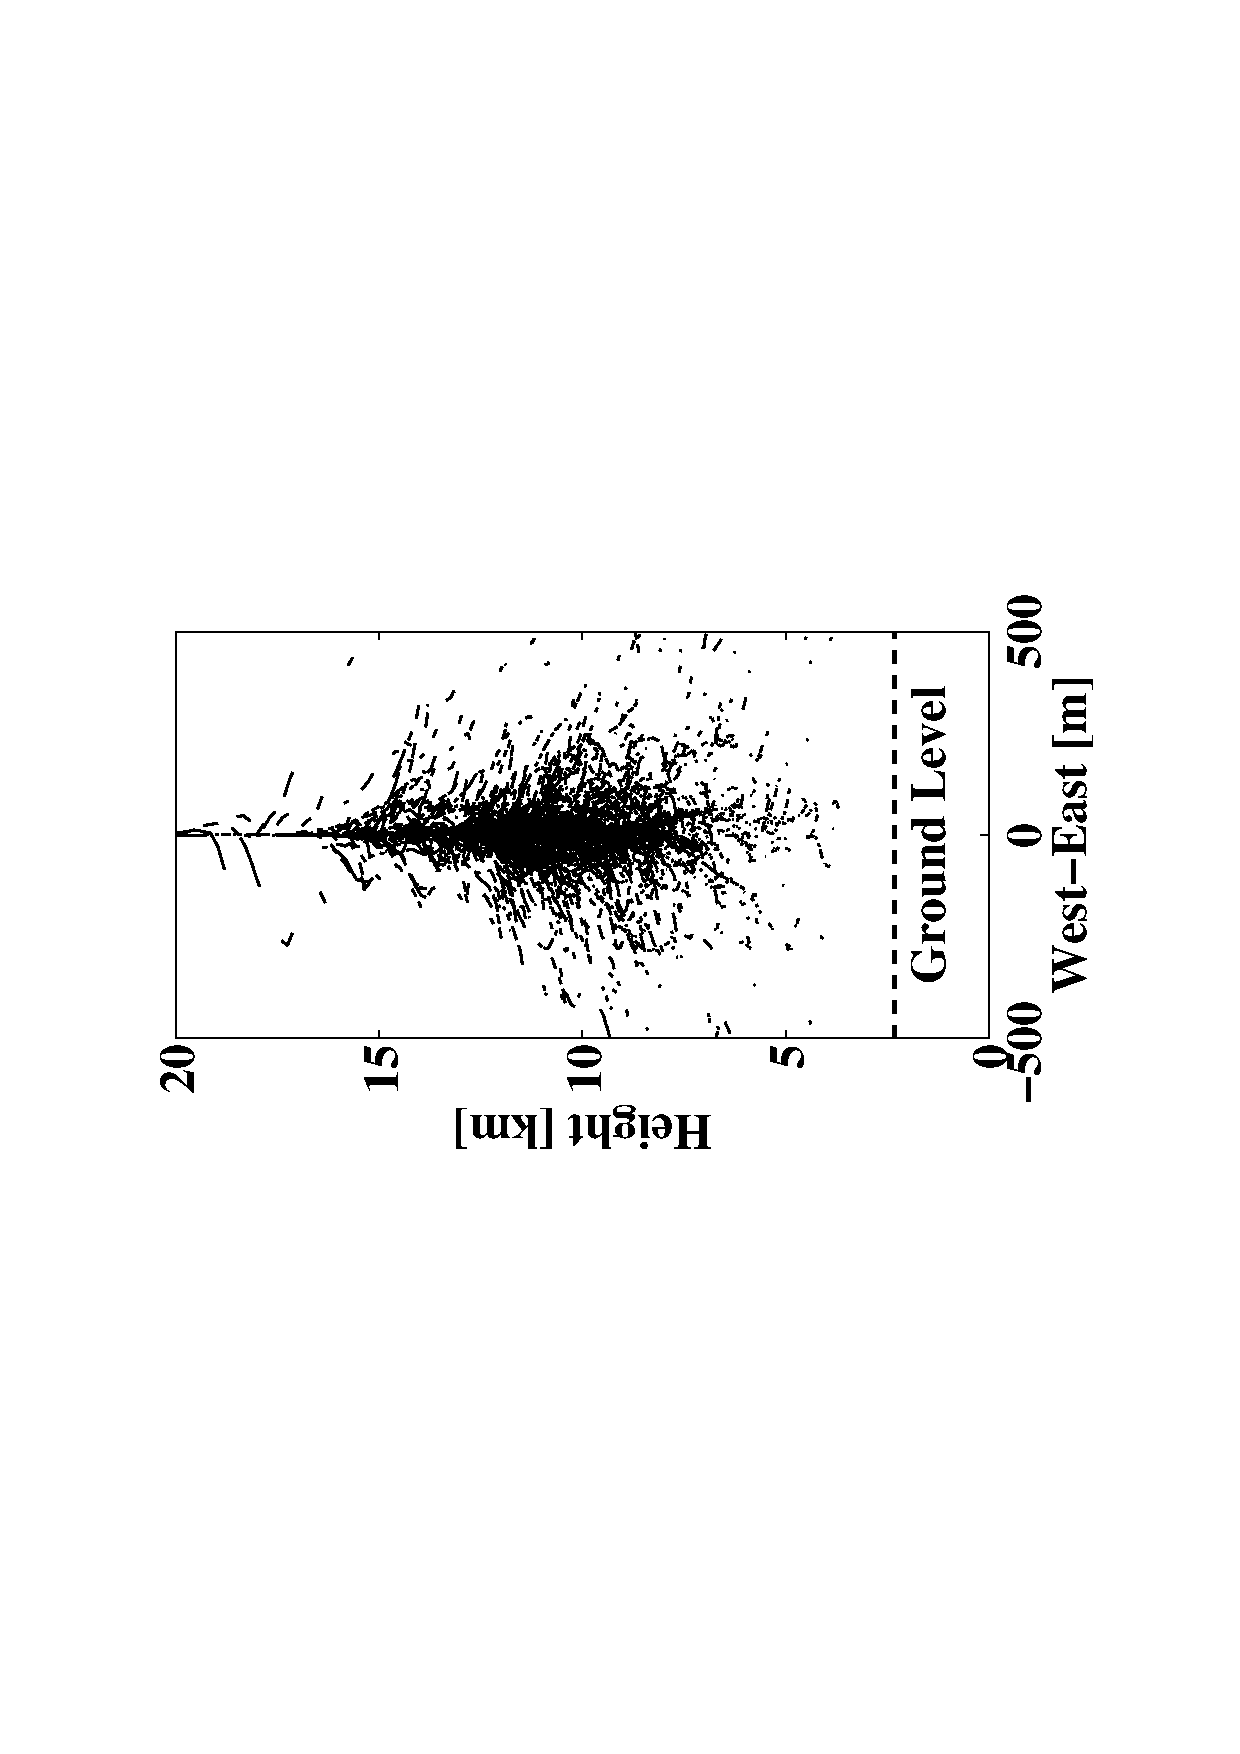
\includegraphics[draft=false]{plots/chap-technique/kas_gamm_100_tr.pdf}}}%
\resizebox*{!}{\textheight}{\rotatebox{270}{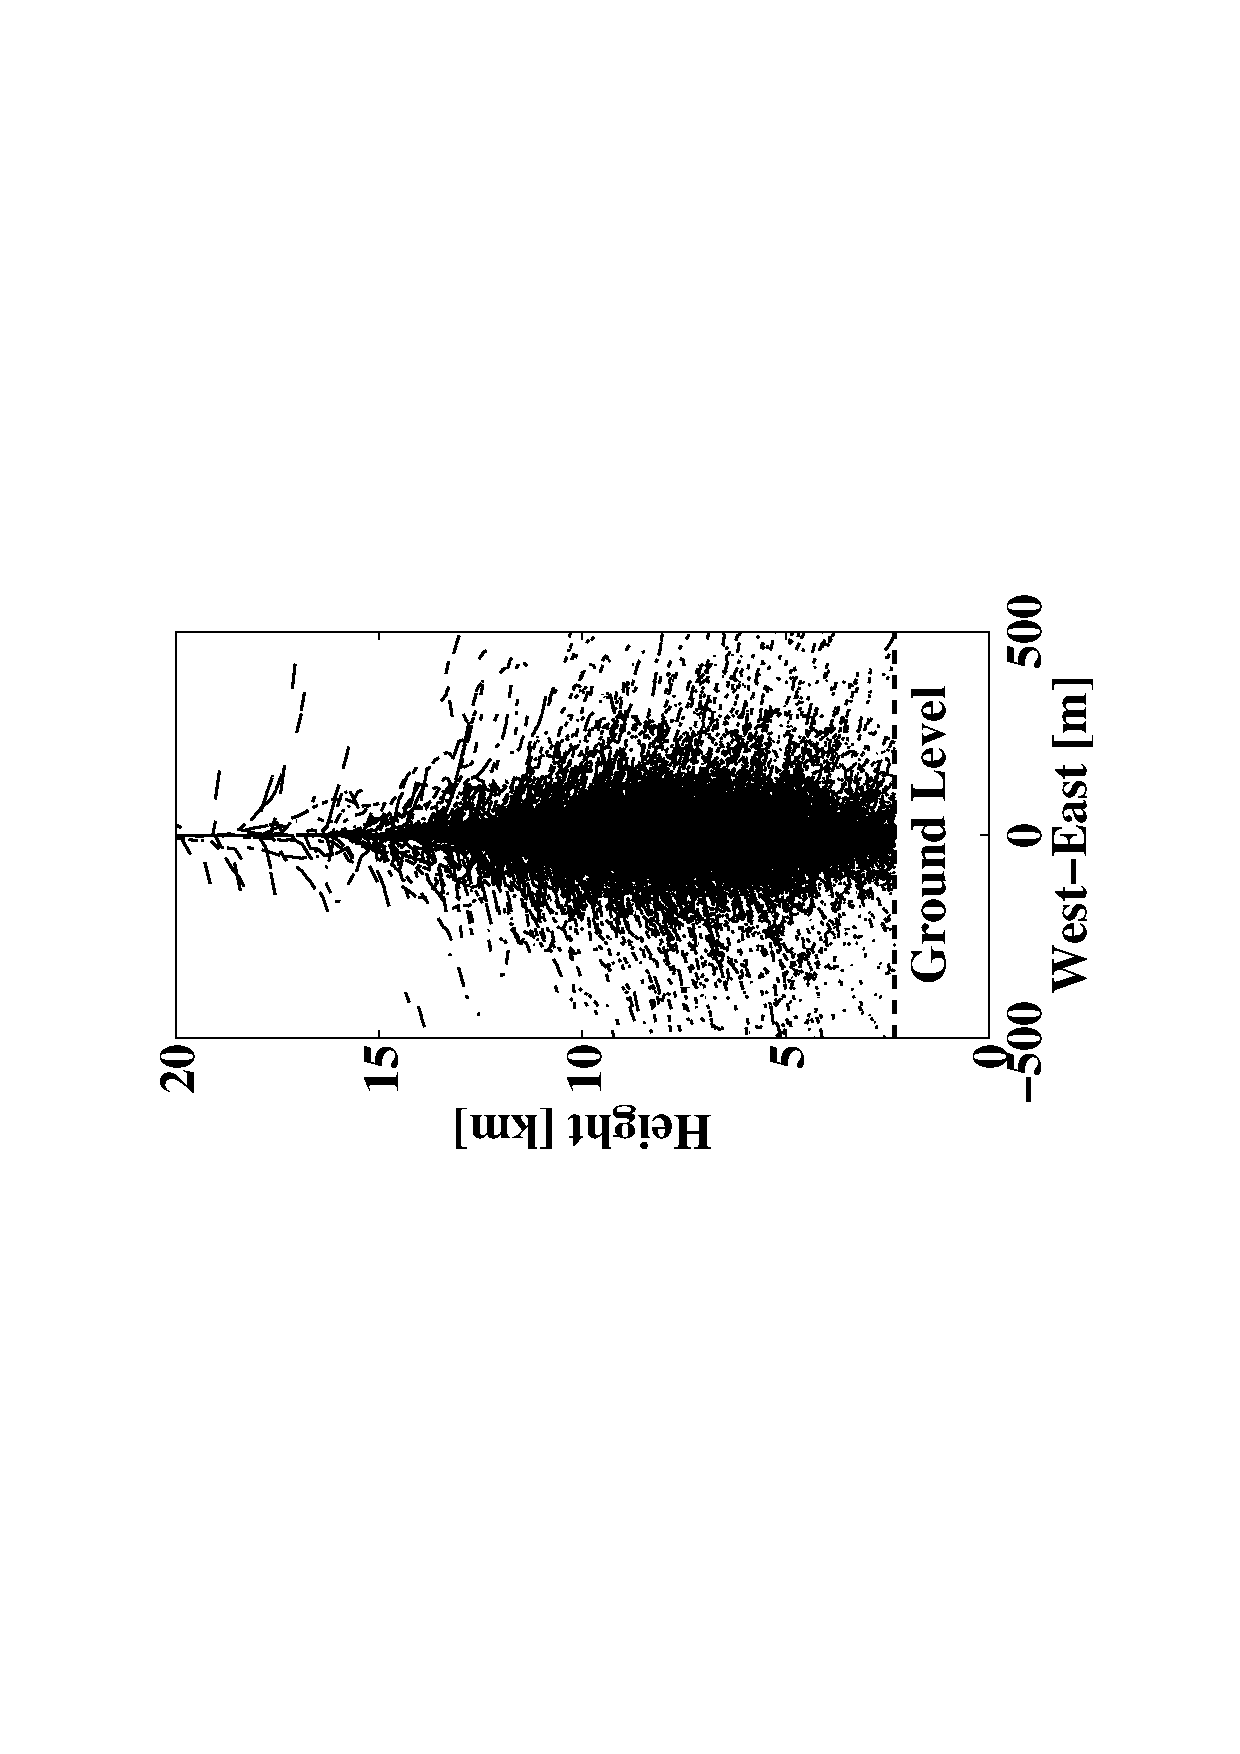
\includegraphics[draft=false]{plots/chap-technique/kas_gamm_1000_tr.pdf}}}%
\resizebox*{!}{\textheight}{\rotatebox{270}{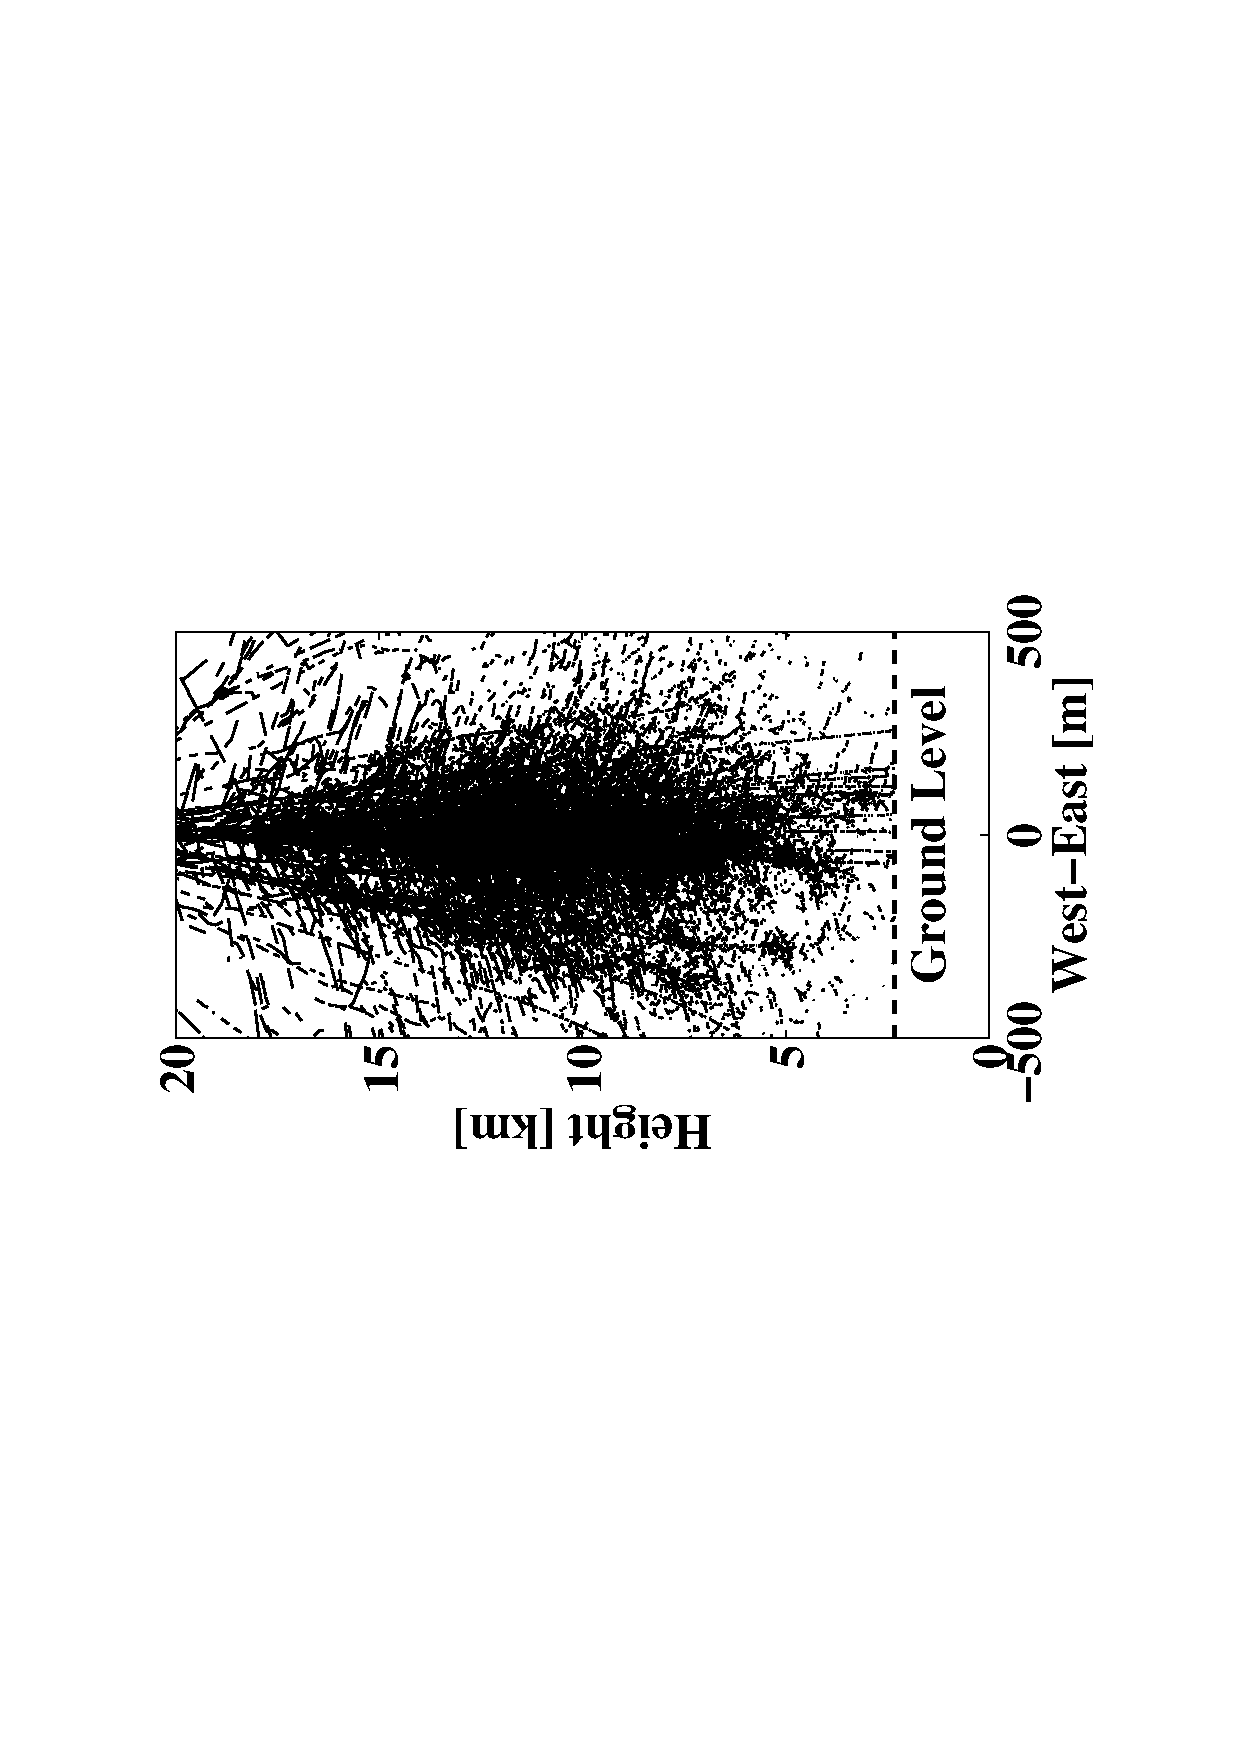
\includegraphics[draft=false]{plots/chap-technique/kas_prot_1000_tr.pdf}}}}}
\caption{\label{FIG::TECHNIQUE::SHOWERS} Simulated charged particle tracks 
in the atmosphere produced by a 100 GeV \Gray (left) and a 1\,TeV
\Gray (middle) and 1\,TeV proton (right). The horizontal and vertical
scales are not equal on this plot. Ground level is set for Mt. Hopkins
at 2320\,m A.S.L.}
\end{figure}

In addition to the electromagnetic component of E.A.S.\ discussed
above, showers initiated by cosmic-rays are dominated by a hadronic
component produced during the initial strong interactions in the upper
atmosphere. These interactions are violent and unpredictable but the
most important end products are neutral and charged pions which decay
to a pair of \Grays or a muon/muon-neutrino pair depending on the
charge of the pion. The
\Gray pairs result in electromagnetic cascades as described above. The
muons, which were identified as a mysterious ``penetrating radiation''
by early cosmic ray researchers, reach the ground with little further
interaction. Since muons take a considerable amount of the energy of
the primary, air-showers produced by hadronic primaries are typically
smaller than those produced by a \Gray of the same energy. Finally,
since the initial strong interactions tend to impart a larger
transverse momentum to the secondaries, a hadronic air-shower will
typically be broader than a \Gray induced shower, consisting of
overlapping cascades produced by different $\pi^0$ particles which
were initially had slightly different directions of propagation. 
Figure~\ref{FIG::TECHNIQUE::SHOWERS} illustrates the distribution of
charged particles in a shower produced by a 1\,TeV proton. Several
muons are visible as straight particle tracks reaching ground level.

\section{Imaging atmospheric \Cerenkov technique}
\label{SEC::TECHNIQUE::IACT}

A third component of all E.A.S.\ is \Cerenkov radiation
\citep{REF::JELLEY::BOOK1958}, produced as
the charged particles in the shower (e$^\pm$ and $\mu^\pm$) traverse
the atmosphere at speeds in excess of the speed of light in
air. \Cerenkov radiation was first noticed in the early 1900s by the
Curies but remained largely a mystery until the 1930s when it was
investigated in a series of experiments which exposed very pure
liquids to $\beta$-radiation \citep{REF::CERENKOV::1934}. The
phenomenon was later explained classically as the coherent
reinforcement of radiation emitted as the charged particle displaces
electrons in the dielectric medium through which it passes
\citep{REF::FRANKTAMM::1937}, work for which the three were awarded
Nobel prizes in 1958. In a tenuous gas medium such as air, where
$n\approx 1-\alpha\rho$ (with $\alpha<<1$) describes the weak
dependence of the index of refraction on the density of the medium,
the \Cerenkov threshold, characteristic angle and intensity of
radiated per unit length of the particle track
\citep{REF::JACKSON::CHAP13} may be written

\centerline{\begin{tabular}{rcll}
$E_t$ & $\propto$ & $\rho^{-1/2}$ & $100-20$\,MeV for e$^-$ between 
25km and sea-level\\
$\theta$ & $\propto$ & $\rho^{1/2}$ & $0.3-1.4^\circ$ \\
$I(\omega)$ & $\propto$ & $\rho$ & $2-30$ photon\,m$^{-1}$ \\
\end{tabular}}

The profile of \Cerenkov light emitted from a very energetic muon
traveling vertically through the atmosphere is illustrated in
figure~\ref{FIG::TECHNIQUE::CERENKOVMUON}. The effect of the changing
atmospheric density along the path of the muon and the resultant
change in the \Cerenkov emission angle causes a focusing of the
\Cerenkov light on the ground and an enhancement of the photon density
at distances of $\sim$120\,m from the muon impact location on the
ground. The photons that strike the ground at distances of $<$30\,m
are due to emission from the region of the atmosphere close to ground
level. The photon density in this region tends to infinity as 1/r
reflecting the essentially constant emission intensity close to the
ground level. Since the atmosphere is a strong absorber of light in
the U.V. region, such ``local'' photons tend to have a spectrum with an
enhanced U.V. component with respect to emission from higher in the
atmosphere. The power of the atmospheric \Cerenkov technique is that a
sufficiently large and sensitive detector can be placed anywhere in
the 45,000\,m$^2$ light pool to detect the particle.

\begin{figure}[t]
\resizebox{\textwidth}{!}{\resizebox*{!}{\textheight}{\rotatebox{270}{\includegraphics{plots/chap-technique/cones.pdf}}}%
\resizebox*{!}{\textheight}{\rotatebox{270}{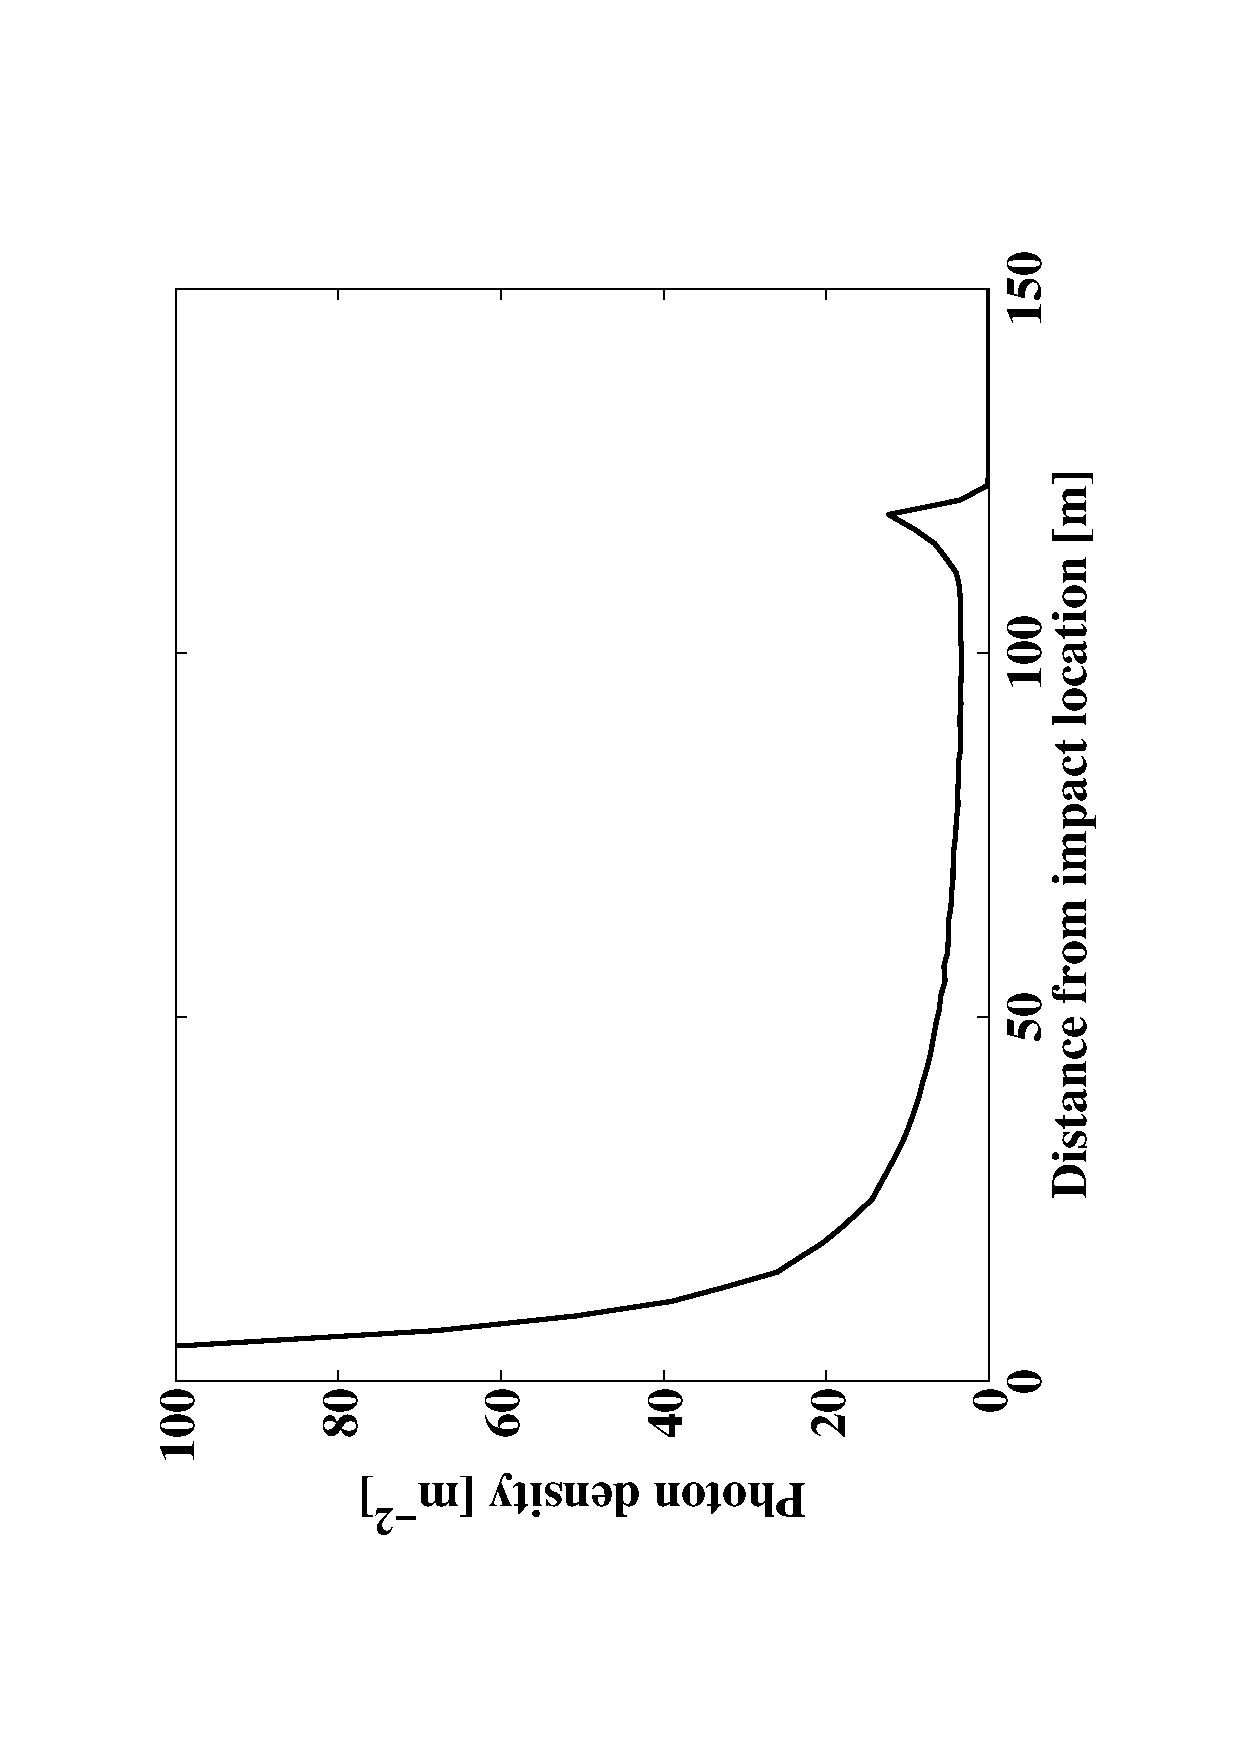
\includegraphics{plots/chap-technique/kas_muon_99999_rd.pdf}}}}
\caption{\label{FIG::TECHNIQUE::CERENKOVMUON} Left: Illustration of 
\Cerenkov emission from vertically moving muon. Right: Radial density 
on the ground of \Cerenkov photons with 200\,nm$<\lambda<$700\,nm,
showing enhancement at 120\,m due to focusing effect of the
increasing atmospheric density. Since the intensity of emitted photons
is essentially constant as the muon reaches the ground, the radial
density diverges like 1/r, as r$\rightarrow$0. }
\end{figure}

The profile of \Cerenkov light from purely electromagnetic air showers
has features similar to the single particle light profile described
above. In general, the transverse momentum (with respect to the
original primary) imparted to the shower particles is small and the
\Cerenkov light pool covers approximately the same area as above.  The
enhancement at 120\,m is also prominent since a considerable amount of
emission comes from the $10-15$\,km region of the atmosphere (see
figure~\ref{FIG::TECHNIQUE::CERENKOVMUON}). At distances greater than
120\,m from the shower core, the fall-off in \Cerenkov density is
slower than single particle case due to multiple Coulomb scattering in
the shower. The \Cerenkov density typically increases with the energy
of the primary as the number of charged particles in the shower core
increases and the development of the shower occurs deeper into the
atmosphere where the density is higher. In addition, the locally
generated \Cerenkov component becomes more significant for larger
showers; a typical 100\,GeV shower, which does not extend to ground
level, will have no local light.

The distribution of \Cerenkov light from hadronically induced showers
is quite different from the electromagnetically induced case above. In
general, a number of muons will be present in the shower which give
rise to considerable local light distributed around their ground
impact locations. Additionally, hadronic showers usually have a number
of EM cascades resulting from decay of different $\pi^0$ particles
which can have considerable transverse momenta. The \Cerenkov light
produced by these photons gives rise to clumps in the distribution on
the ground. In some small fraction of cases most of the energy of the
primary can go to a single $\pi^0$ and an essentially electromagnetic
shower can arise with properties almost identical to {\Grayc}-induced
showers. Finally, in the hadronic case, there tends to be a large
variance in the profile of showers triggered by identical primaries,
due to the initial strong force interactions.

The detection of \Cerenkov light from air-showers was pioneered by
\citet{REF::GALBRAITHJELLEY::1953, REF::GALBRAITHJELLEY::1955} using a
ten inch mirror with photomultiplier tube at its focus. Since these
early experiments, the desire to discriminate {\Grayc}-induced
air-showers from the overwhelming background of hadronic showers has
largely driven the design of atmospheric \Cerenkov instruments. The
development of the imaging technique by the Whipple collaboration
yielded the first detection of very high energy \Gray emission from an
astronomical source \citep{REF::WEEKES::APJ1989}. The essence of the
imaging technique is to take a snapshot of the \Cerenkov flash
associated with the air-shower using a high resolution camera system
consisting of an array of close packed photo-tubes mounted at the focus
of a large telescope, fast triggering and readout electronics to
digitize the $\sim$10\,ns signals and a data acquisition system capable
of recording the data with a minimum of dead time. 

\begin{figure}[t]
\centerline{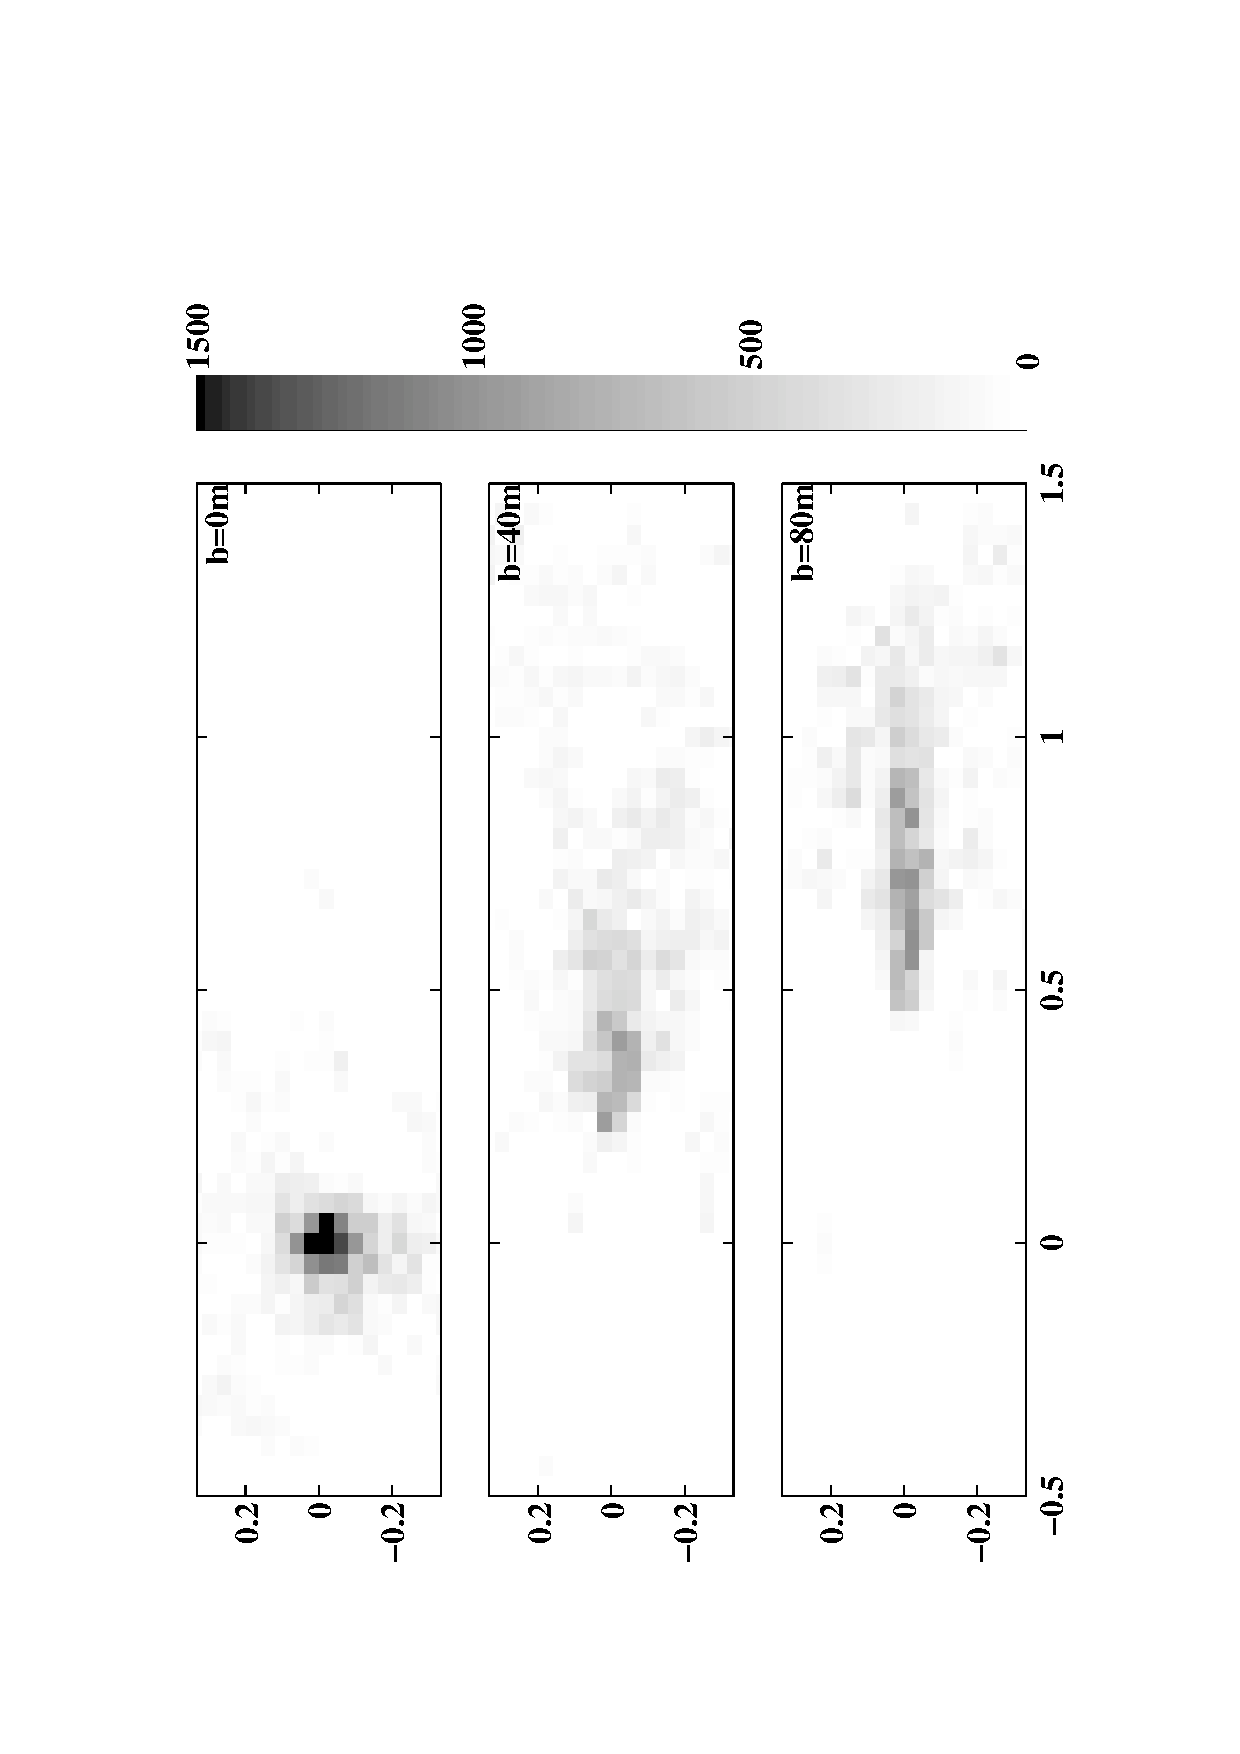
\includegraphics[angle=270,width=0.65\textwidth]{plots/chap-technique/fplane_density.pdf}}
\caption{\label{FIG::TECHNIQUE::FPDENSITY} Density of photons per 
unit mirror area in the focal plane of an ideal 10\,m telescope for a
simulated 350\,GeV photon induced shower, in units of
m$^{-2}$\,deg$^{-2}$. The same shower is shown for three different
impact parameters: 0\,m, 40\,m and 80\,m. The axes gives the angular
distance in the focal plane from the direction of the primary (which
is assumed to be coincident with the center of the camera) in
degrees.}
%The shading scale does not fully
%accomodate the density of the brightest bins in the $b=0$ image, which
%contains considerable local light.}
\end{figure}

In the focal plane of such an instrument, the image traces the
development of the shower in the sky. For an EM induced shower the
image is largely symmetric around the projection of the shower axis
onto the field of view of the instrument, reflecting the symmetry of
the shower itself around the axis. The images of EM showers are often
described as ``cometary''; one side of the shower, in the direction of
towards the early stages of the shower development (i.e.\ towards the
upper atmosphere) has a higher photon density. As the shower dies
after shower maximum, the image becomes more diffuse with a lower
photon density, spread out over a larger area of the image.  Higher
energy showers produce more secondaries, more \Cerenkov photons and
extend further into the atmosphere, resulting in an image which has a
larger photon density and a larger extent in the field of view.
Finally the appearance of the shower in the field of view is dependent
to a large extent on the distance between the shower axis and the
instrument, usually called the \textit{impact parameter} and denoted
as $b$. Figure~\ref{FIG::TECHNIQUE::FPDENSITY} illustrates an image of
a 350\,GeV \Gray shower viewed at three different impact parameters.
The showers become elongated and displaced from the center of the
camera as the impact parameter increases. Images of proton induced
showers are less compact than \Gray showers, due largely to the higher
transverse momentum imparted by the strong interactions. Data
selection criteria, based on these differences, capable of keeping a
large fraction of the \Gray events while discarding the majority of
the background cosmic-ray events are described in
chapter~\ref{CHAP::ANALYSIS}.

\section{Trigger and acquisition electronics}
\label{SEC::TECHNIQUE::ELECTRONICS}

\begin{figure}[p]
\centerline{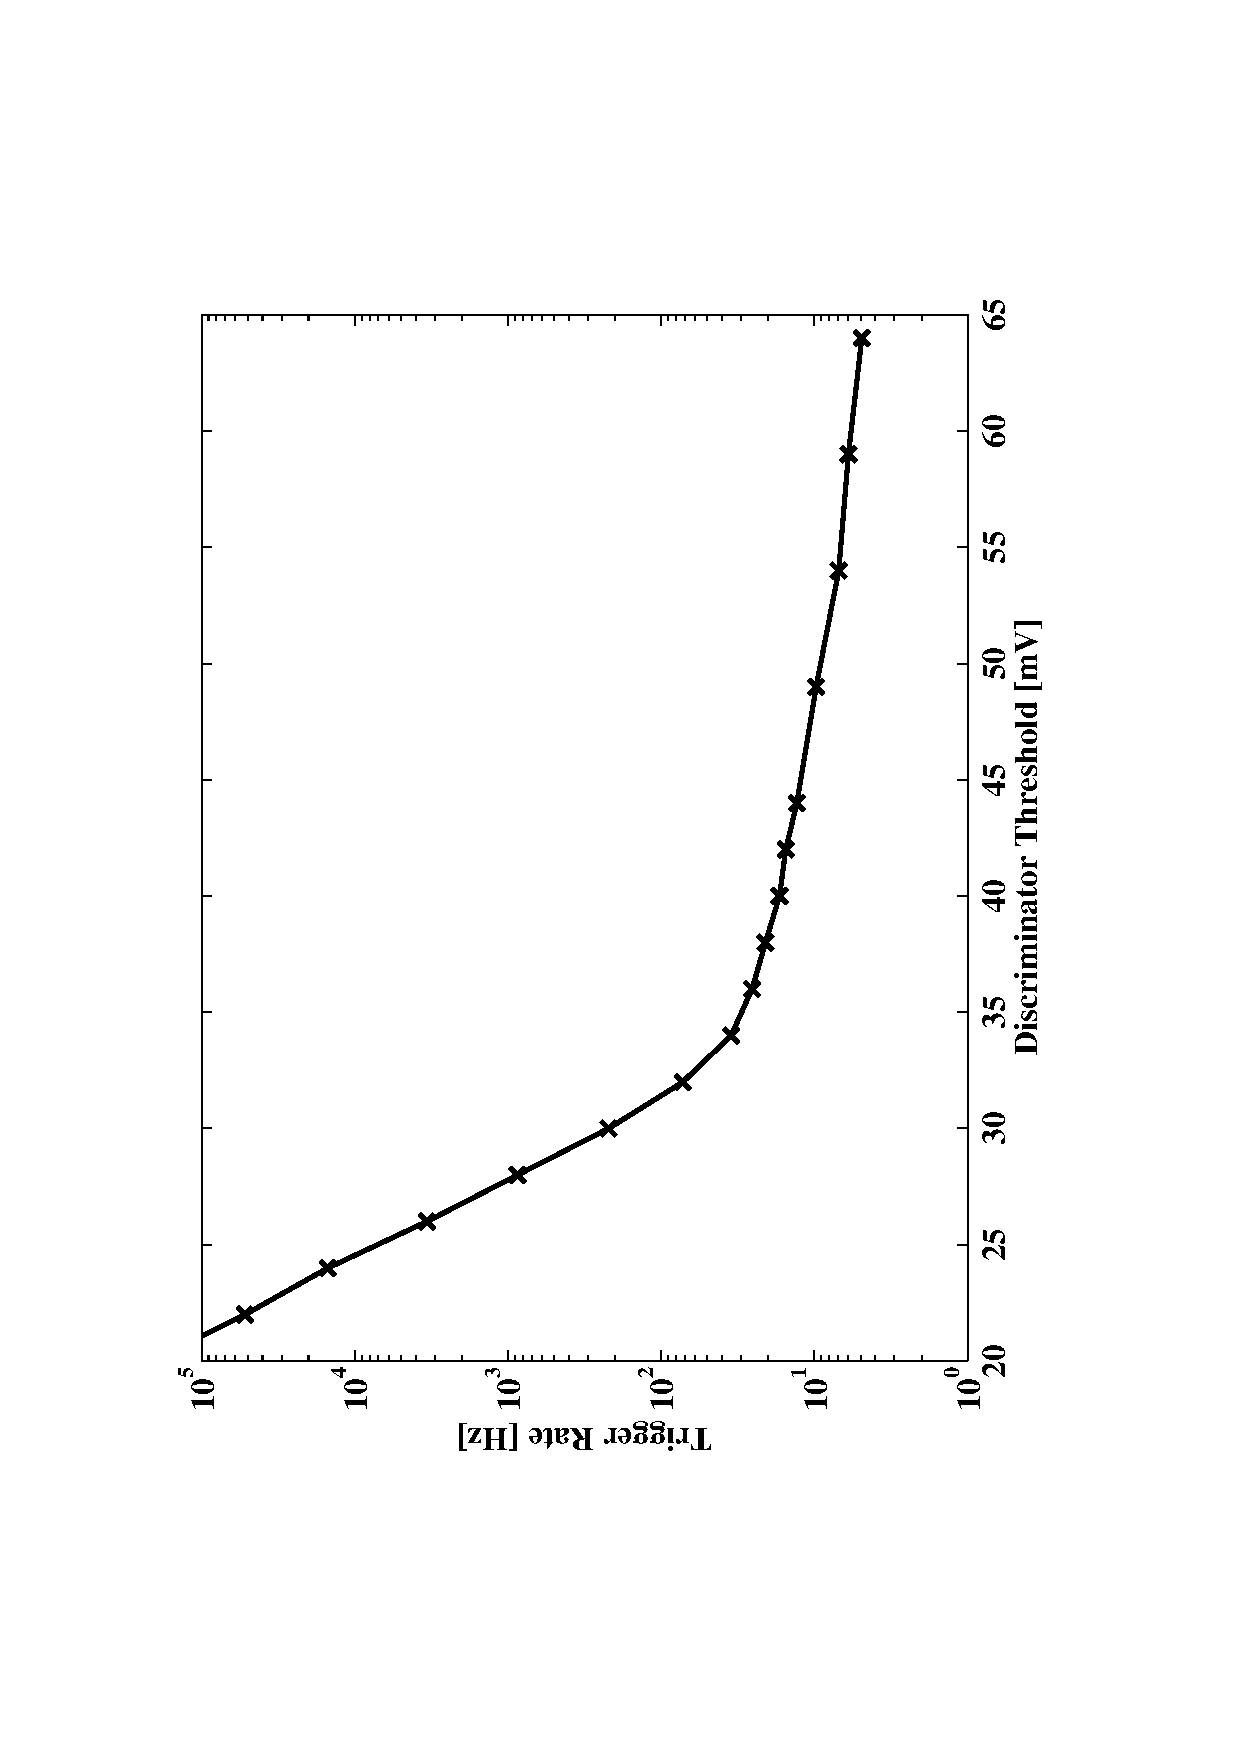
\includegraphics[angle=270,width=0.7\textwidth]{plots/chap-technique/bias_011009.pdf}}
\caption{\label{FIG::TECHNIQUE::BIASCURVE} Event rate vs.\ L-1
trigger threshold with a trigger L-2 requirement (pattern selection
trigger) of three adjacent channels exceeding the threshold within the
coincidence time. This kind of plot is usually referred to as a ``bias
curve''.}
\end{figure}

\begin{figure}[p]
\centerline{\includegraphics[width=0.7\textwidth]{plots/chap-technique/el_schematic.pdf}}
\caption{\label{FIG::TECHNIQUE::ELSCHEMATIC} Schematic of the major
components of the data acquisition system. See text for discussion.}
\end{figure}

Readout of the 379 channel camera is initiated by a two-level trigger
system. At the lowest level (L-1), each of the inner 331 channels are
monitored by a constant fraction discriminator (CFD), which triggers
when the signal exceeds a pre-programmed level. For a constant pulse
profile, the CFD compensates for the time jitter intrinsic to a
standard discriminator (i.e.\ simple voltage comparator), which
triggers earlier, relative to the peak in the pulse profile, for
signals with large amplitude. The digital outputs of these CFDs are
then processed by the second level of trigger (L-2), an electronic
system referred to as the \textit{pattern selection trigger} or
PST\footnote{Actually, there are two separate electronic systems
involved in the L-2 trigger. The second system, called the
multiplicity trigger, has very little time jitter in comparison to the
PST, and is used only to set the timing of the L-2 output.}, which is
essentially a memory lookup table that can be programmed to
discriminate images with two, three or four adjacent channels from
those where the triggering channels are non-adjacent. This trigger
design, which preferentially records images of compact \Gray and
hadronic showers over the random fluctuations of the night-sky
background, is described in detail in
\citet{REF::BRADBURY::1999SLC}. In general it is desirable to set the
discriminator threshold as low as possible, allowing lower energy
events to be recorded. At low trigger levels, the night-sky background
light causes an excessive event rate, even with the PST. The trigger
is set to ensure that the event rate is below the maximum sustainable
rate of the data acquisition system, $\sim35$\,Hz, even when observing
the brightest fields of view. Figure~\ref{FIG::TECHNIQUE::BIASCURVE}
shows the trigger rate vs.\ trigger threshold, as measured in late
2001. At high thresholds, the rate is dominated by the power-law
cosmic-ray spectrum; below approximately 35\,mV the rate curve becomes
very steep, due to random triggers by night-sky noise. A setting of
$\sim38$\,Hz would result in a relatively stable rate, even under the
brightest of conditions.

A schematic of the main components of the data acquisition system is
shown in figure~\ref{FIG::TECHNIQUE::ELSCHEMATIC}. The signal from
each channel, after $\times10$ amplification, is digitized by a set of
LeCroy 2249A 0.25\,pC/count charge-to-digital converters (QADC).
Conversion is initiated by the L2 trigger; in order to allow for the
trigger decision to be formed, the signals are delayed in a length of
RG-58 cable, allowing the trigger decision and signals from the PMTs
to reach the ADCs coincidentally. The integration time of $\sim$20\,ns
is longer than the intrinsic duration of the \Cerenkov flash on the
ground, in order to account for the time-spread introduced by the
spherical mirror (see figure~\ref{FIG::INTRODUCTION::SCOPE}) and
dispersion in the delay cables. As a consequence, more night-sky noise
is integrated in the signal that would otherwise be the case. Future
experiments will minimize this noise by having mirrors with longer
focal lengths (hence smaller time-spreads) and by eliminating the need
for long signal delay cables using electronic delay systems. One
approach to the latter is to continually sample the signal with flash
ADCs, storing the digitized information in a temporary RAM buffer
which can then be read out when the trigger decision is made.

The signal is AC coupled at the input of the amplifier to remove any
bias current through the tube, due mainly to the night-sky brightness
that the tube is exposed to in addition to the (significantly smaller)
dark current in the tube. A small biasing, or pedestal, current is
then reintroduced to the signal in the input stage of the QADCs to
facilitate the measurement of negative fluctuations of the signal from
the mean sky-brightness. This biasing current is removed during the
analysis of the data, as described in
section~\ref{SUBSEC::ANALYSIS::PEDESTAL}. The data is read out over a
computer network and stored on disk for offline analysis.

It is estimated that a single photo-electron in the PMTs produces a
signal of $\sim3.3$\,counts in the QADC. This corresponds to a total
gain in the system of $\sim5\times10^{6}$.

\section{Characterization of detector}
\label{SEC::TECHNIQUE::CHARACTERISTICS}

Unlike the lower energy satellite based \Gray instruments, the
response of a ground-based \Cerenkov telescopes cannot be measured
using an artificial test beam. Characterization of the response of
such instruments to \Grays and cosmic-rays must be done using
simulations, by modeling the air-shower development, \Cerenkov light
production and detector response. For such a study to be accurate, the
simulations must correctly account for such factors as: nuclear
physics cross-sections (especially for hadronic simulations),
atmospheric density profile and response to \Cerenkov radiation,
wavelength dependent mirror reflectivity and PMT quantum efficiency,
dispersion in the cables, response of the trigger and ADCs, and
others. Many of these can be accurately measured in the laboratory,
others must be extrapolated from standard tables, such as the U.S.\
standard atmosphere model. It is estimated that the accuracy of such a
simulation study $\sim20$\%. This is borne out by the impressive
agreement in the spectrum of the Crab Nebula source calculated, from
observations, by the various ground-based VHE observatories in the
northern hemisphere, such as Whipple, HEGRA and CAT. These groups
employ different simulation codes, both for shower physics and
detector simulation, yet derive spectra for the Crab that agree to
within the limits of statistical and systematic errors.

Chapter~\ref{CHAP::VERITAS} describes the study of a next generation
ground-based instrument, VERITAS, in some detail. The results of a
similar study of the Whipple telescope are presented here, with a
brief description of the simulations.

The KASCADE simulation package \citep{REF::KERTZMAN::1994NIMA} was used
to generate sets of {\Grayc}-induced air shower events. Sets of
{\Gray}-induced events were generated over a range of energies between
30\,GeV and 30\,TeV. The energy bins were evenly distributed in $\log
E$ with eight bins per decade of energy. To accommodate the decreasing
detection efficiency of the instrument at lower energies, the number
of events simulated per bin was chosen to increase sharply at lower
energies, to ensure that sufficient events were available so that some
of them would survive the simulated trigger requirements and data
selection procedure.

For each event, the \Cerenkov photons generated in the shower were
traced to see whether they intersected the mirror. The wavelength
dependent reflectivity was accounted for and, if the photon was
reflected into a PMT, so also was the quantum efficiency of the tube.
The resultant photo-electrons produced by the shower (if there were
any) were combined with artificially generated, Poisson distributed,
night-sky photo-electrons, producing a realistic image that is
comparable to an image of a real \Grayc. The images were subjected to
the standard trigger requirement of three neighboring channels above a
threshold of $\sim7$ photo-electrons. Those events that pass the
trigger requirement are then processed using the standard analysis and
data selection criteria, as described in chapter~\ref{CHAP::ANALYSIS}.
Figure~\ref{FIG::TECHNIQUE::AREA_DRDE} shows the simulated response of
the instrument to on-axis \Gray primaries at an angle of $20^\circ$
to the zenith. For a Crab Nebula like spectrum (power law --
$dF/dE\propto E^{-2.5}$) the instrument is most sensitive to \Grays
with energy of $\sim$350\,GeV. It is usual to refer to this as the
\textit{peak response energy} of the instrument\footnote{Or somewhat
incorrectly, as the \textit{energy threshold} of the instrument.} and
to quote fluxes and upper-limits measured with the instrument at that
energy.

\begin{figure}[t]
\centerline{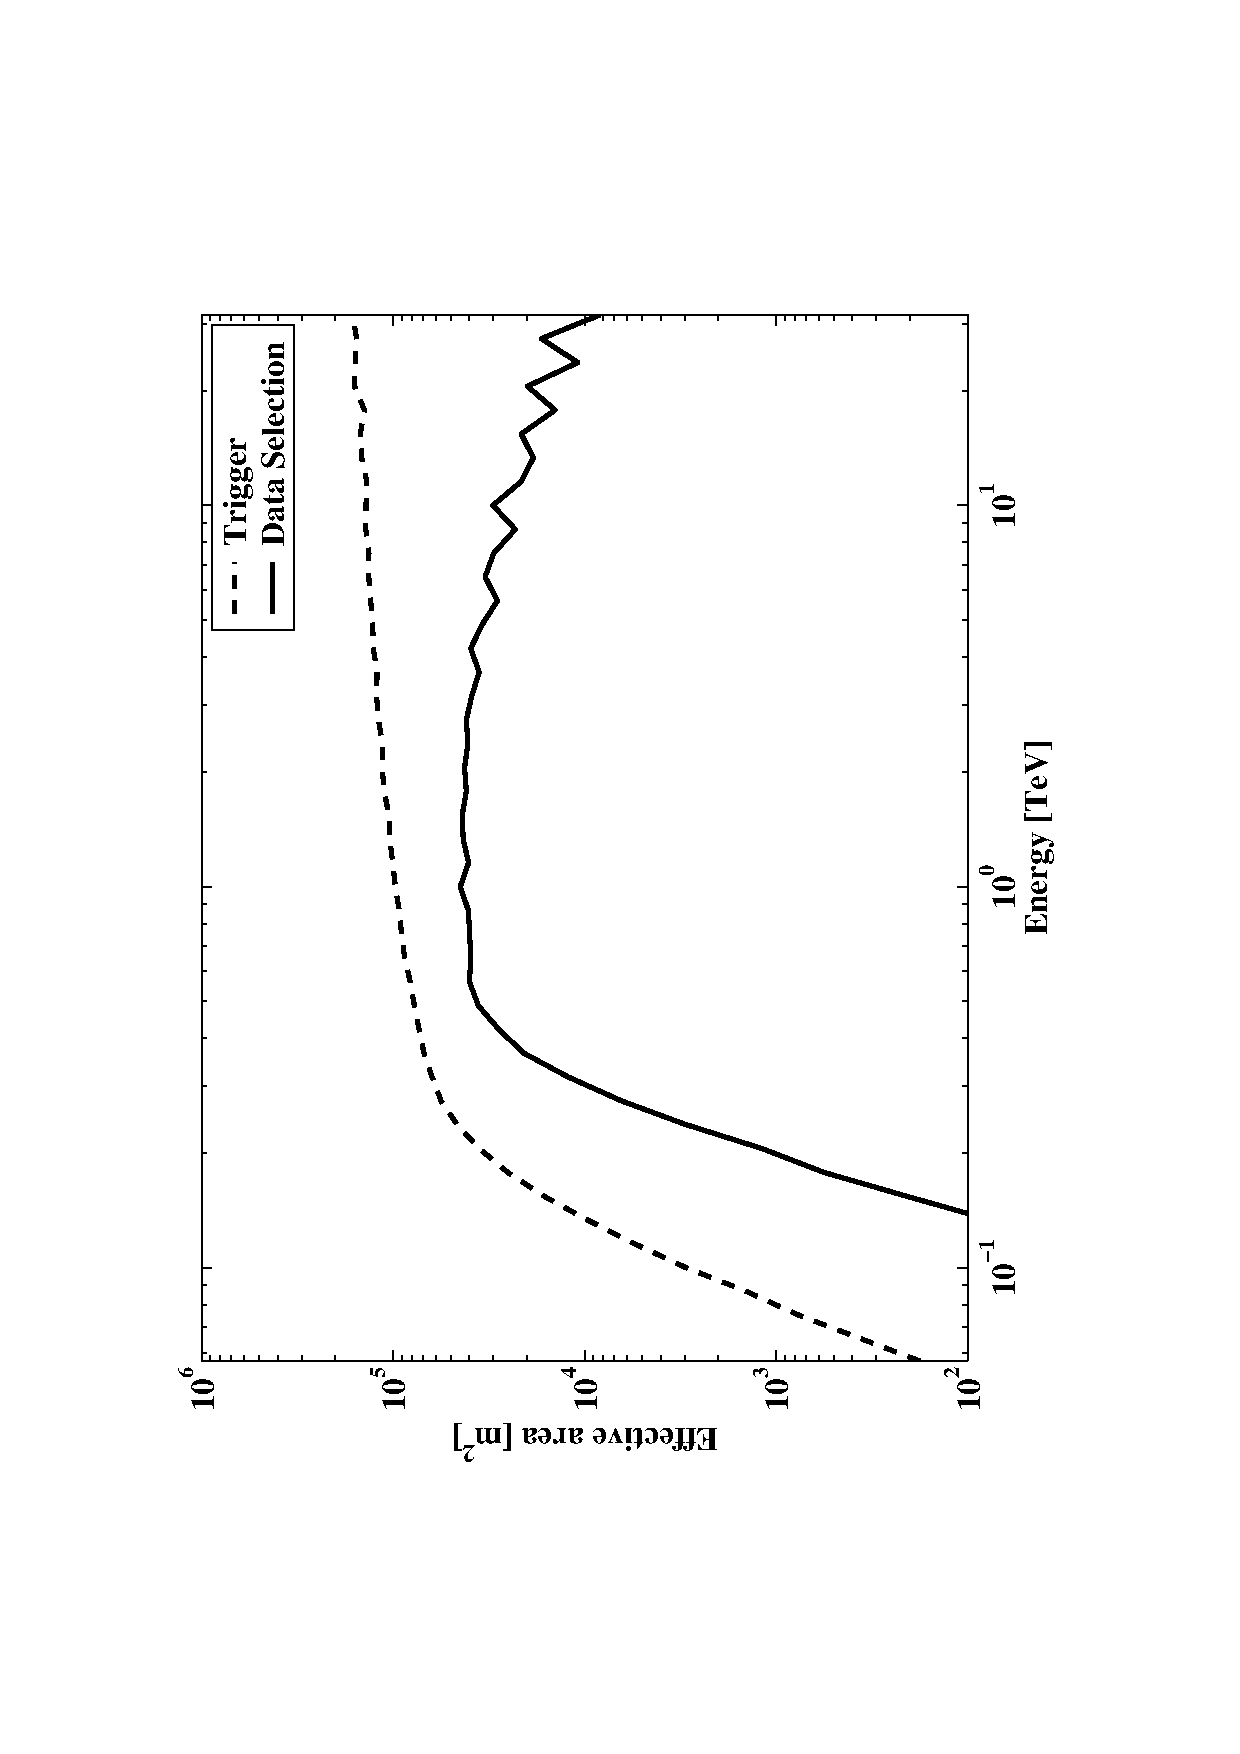
\includegraphics[angle=270,width=0.49\textwidth]{plots/chap-technique/detector_response_area.pdf}\includegraphics[angle=270,width=0.49\textwidth]{plots/chap-technique/detector_response_drde.pdf}}
\caption{\label{FIG::TECHNIQUE::AREA_DRDE} (Left) Effective
collection area vs.\ energy for trigger and for data selection
algorithm. After data selection, the collection area peaks at
$\sim4\times10^4$\,m$^2$. (Right) Differential rate of \Grays
collection from Crab Nebula. } \end{figure}

